\documentclass[10pt,t]{beamer} % handout
\usetheme{Heverlee}
\usepackage{animate}
\usepackage{tikz}
\usepackage{tikz-cd}
\usepackage{svg}

\newcommand{\R}{\mathbb{R}}

\newenvironment<>{varblock}[2][\textwidth]{%
	\setlength{\textwidth}{#1}
	\begin{actionenv}#3%
		\def\insertblocktitle{#2}%
		\par%
		\usebeamertemplate{block begin}}
	{\par%
		\usebeamertemplate{block end}%
\end{actionenv}}

\setbeamertemplate{theorems}[numbered] 
\newtheorem{result}{Result}

%%% QUICK OPTIONS:
% (A) Math font without serifs, enable line below to make math serif:
    \usefonttheme[onlymath]{serif}

% (B) Re-define primary colour by adjusting the RGB values
%    \definecolor{pblue}{RGB}{206,125,66}

% (C) Title page graphic (optional) --- this is not for the background image, see \usebackgroundtemplate to change that ---
    %\titlegraphic{\includegraphics[height=2.7cm]{example_figure.pdf}}

% (D) Add logo to bottom right-corner (optional)
    \logo{\includegraphics[height=0.7cm]{icosahedron-src.pdf}\hspace{12pt}\vspace{-6pt}} 

% (E) Choose one (or none) of these lines to add footline bar on all frames
    %\setbeamertemplate{footline}[infoline]  % author, title, insitute
    %\setbeamertemplate{footline}[navigation] % dots swhowing progress
    %\setbeamertemplate{footline}[navsym] % navigation symbols

% (F) Widescreen 16:9 ratio
    %\usepackage[orientation=landscape,size=custom,width=16,height=9,scale=0.45,debug]{beamerposter} 


%%% TITLE PAGE INFO:

\title{Derived Commutativity in Data Science,\\ Category Theory, and Quantum Physics}
\subtitle{Theoretical and computational aspects}
\author[ammedmar]{Anibal M. Medina-Mardones}
\institute{Max Planck Institute for Mathematics}
\date{March 2021}

\begin{document}
{
% Change image, or delete this line to remove background image
\usebackgroundtemplate{ \parbox[b][\paperheight][b]{\paperwidth}{\centering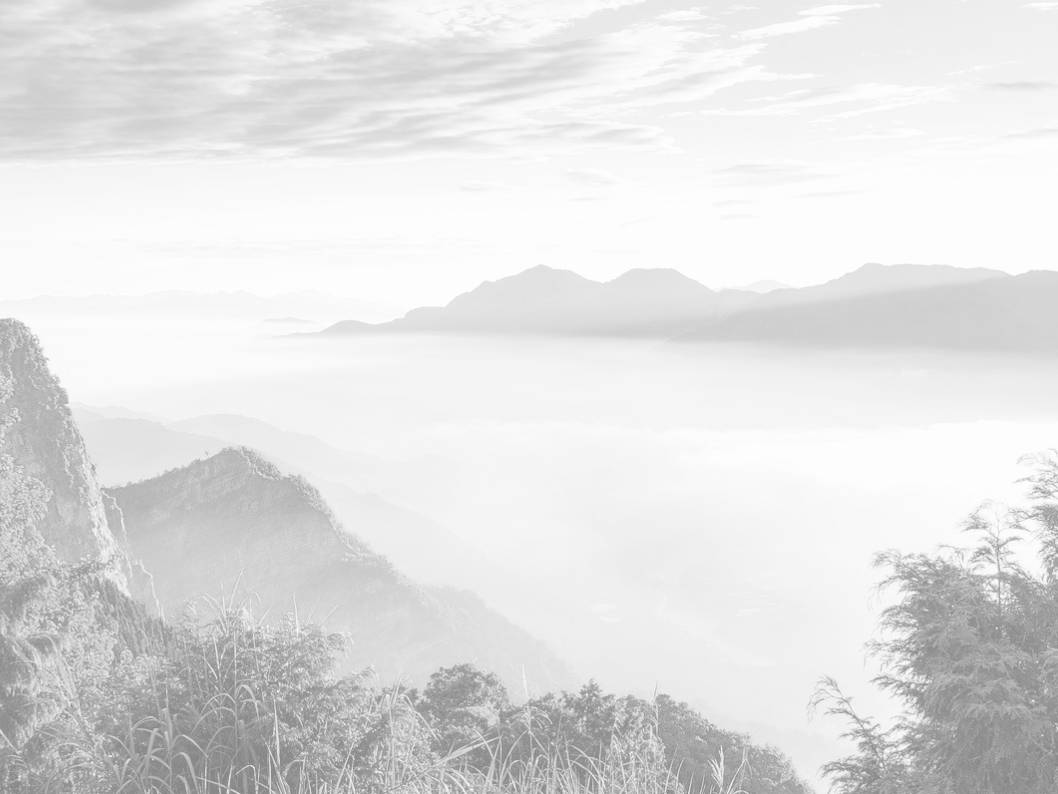
\includegraphics[width=\paperwidth]{bg_alishan.jpg}}} 
 %   abudhabi      cherry      forest      river
 %   alishan       chobe       leuven      sanfancisco
 %   blueprint     columns     library     uyuni
 %   bokeh         flowers     newyork     winter

%\setbeamercolor{background canvas}{bg=lgray}  % make background light gray

% Title page
\begin{frame}[plain, noframenumbering]
    \titlepage
\end{frame}
}

% Table of contents slide
\begin{frame}{Outline}
	\vskip 2mm
	\hfill	{\large \parbox{.95\textwidth}{\tableofcontents[hideothersubsections]}}
\end{frame}

\section{From data to topology}

\begin{frame}{Point clouds}
	\begin{itemize}
		\item A data set can often be thought of as a point cloud in $\R^n$.
		
		\vskip 8pt
		\pause
		
		\item Underlying probability distribution concentrated in a subspace.
		
		\vskip -5pt
		
		\begin{center}
			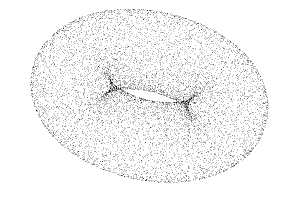
\includegraphics[scale=.3]{torus}
		\end{center}
		
		\pause 
		
		\item How to approximate and study the underlying shape?
		
		\pause
		\vskip 5pt
		
		\begin{center}
			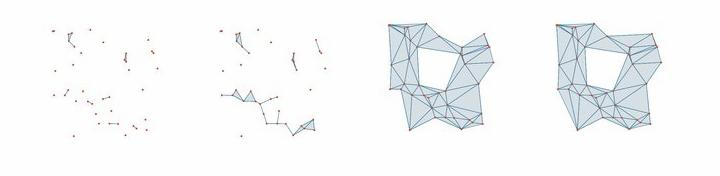
\includegraphics[scale=.4]{filtration}
		\end{center}
	
		\vskip -3pt
		
		Approximate using a multiscale construction.
	\end{itemize}
\end{frame}

\begin{frame}{Persistence homology}	
	\begin{itemize}
		\item Study through construction of invariants of the associated shapes.
		
		\pause
		
		\item Topology provides principled ways of constructing invariants.
		
		\vskip 10pt
		\begin{center}
			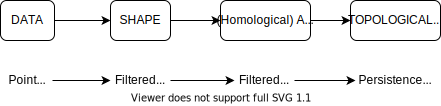
\includegraphics[scale=.5]{diagram}
		\end{center}
	
		\pause
		\item \textcolor{pblue}{Machine Learning Intuition}: The 0-dimensional part of this invariant is equivalent to hierarchical clustering.
		
		\begin{center}
			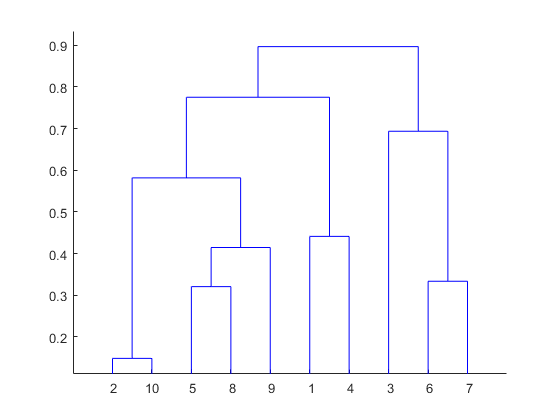
\includegraphics[scale=.2]{dendogram}
		\end{center}
	\end{itemize}	
\end{frame}

\begin{frame}{Machine Learning and Topology}
	Is there a way for ML practitioners to easily incorporate persistence homology into standard pipelines?
	
	\vskip 10pt
	\pause
	\includegraphics[scale=.31]{giotto}	
\end{frame}

\section{Finer invariants}

\begin{frame}{Finer topological invariants}
	\newcommand*{\xMin}{0}%
	\newcommand*{\xMax}{4}%
	\newcommand*{\yMin}{0}%
	\newcommand*{\yMax}{4}%
	\begin{center}
	\begin{tikzpicture}[scale=.6]
	\draw[-{Latex[length=2mm]}] (-.5,\yMin)--(-.5,\yMax);
	\draw[-{Latex[length=2mm]}] (-.5,\yMin)--(-.5,\yMax-.5);
	\draw[-{Latex[length=2mm]}] (4.5,\yMin)--(4.5,\yMax);
	\draw[-{Latex[length=2mm]}] (4.5,\yMin)--(4.5,\yMax-.5);
	
	\draw[-{Latex[length=2mm]}] (\xMin, -.5)--(\xMax, -.5);
	\draw[-{Latex[length=2mm]}] (\xMin, 4.5)--(\xMax, 4.5);
	
	\draw (0,0)--(0,4)--(4,4)--(4,0)--(0,0);
	
	\node at (2,-1.2){$T$};
	\end{tikzpicture}
	\hspace*{2cm}
	\begin{tikzpicture}[scale=.6]
	\draw[-{Latex[length=2mm]}] (-.5,\yMin)--(-.5,\yMax);
	\draw[-{Latex[length=2mm]}] (-.5,\yMin)--(-.5,\yMax-.5);
	\draw[-{Latex[length=2mm]}] (4.5,\yMax)--(4.5,\yMin);
	\draw[-{Latex[length=2mm]}] (4.5,\yMax)--(4.5,\yMin+.5);
	
	\draw[-{Latex[length=2mm]}] (\xMin, -.5)--(\xMax, -.5);
	\draw[-{Latex[length=2mm]}] (\xMin, 4.5)--(\xMax, 4.5);
	
	\draw (0,0)--(0,4)--(4,4)--(4,0)--(0,0);
	
	\node at (2,-1.2){$K$};
	\end{tikzpicture}
	\end{center}
\end{frame}

\begin{frame}{Finer topological invariants}
	\newcommand*{\xMin}{0}%
	\newcommand*{\xMax}{4}%
	\newcommand*{\yMin}{0}%
	\newcommand*{\yMax}{4}%
	
	\begin{center}
	\begin{tikzpicture}[scale=.6]
	\draw[-{Latex[length=2mm]}] (-.5,\yMin)--(-.5,\yMax);
	\draw[-{Latex[length=2mm]}] (-.5,\yMin)--(-.5,\yMax-.5);
	\draw[-{Latex[length=2mm]}] (4.5,\yMin)--(4.5,\yMax);
	\draw[-{Latex[length=2mm]}] (4.5,\yMin)--(4.5,\yMax-.5);
	
	\draw[-{Latex[length=2mm]}] (\xMin, -.5)--(\xMax, -.5);
	\draw[-{Latex[length=2mm]}] (\xMin, 4.5)--(\xMax, 4.5);
	
	\draw (0,0)--(0,4)--(4,4)--(4,0)--(0,0);
	
	\draw[color=blue!50, very thick] (0,2) .. controls (1,2.5) and (3,1.5) .. (4,2);
	\draw[color=red!50, very thick] (0,1) .. controls (1,1.3) and (3,1) .. (4,1);
	
	\node at (2,-1.2){$T$};
	\end{tikzpicture}
	\hspace*{2cm}
	\begin{tikzpicture}[scale=.6]
	\draw[-{Latex[length=2mm]}] (-.5,\yMin)--(-.5,\yMax);
	\draw[-{Latex[length=2mm]}] (-.5,\yMin)--(-.5,\yMax-.5);
	\draw[-{Latex[length=2mm]}] (4.5,\yMax)--(4.5,\yMin);
	\draw[-{Latex[length=2mm]}] (4.5,\yMax)--(4.5,\yMin+.5);
	
	\draw[-{Latex[length=2mm]}] (\xMin, -.5)--(\xMax, -.5);
	\draw[-{Latex[length=2mm]}] (\xMin, 4.5)--(\xMax, 4.5);
	
	\draw (0,0)--(0,4)--(4,4)--(4,0)--(0,0);
	
	\draw[color=blue!50, very thick] (0,2) .. controls (1,2.5) and (3,1.5) .. (4,2);
	\draw[color=red!50, very thick] (0,1) .. controls (1,1) and (2,2.5) .. (4,3);
	
	\node at (2,-1.2){$K$};
	\end{tikzpicture}
	\end{center}
	
	Although $H^\bullet(T, \mathbb F_2) \cong H^\bullet(K, \mathbb F_2)$ as graded vector spaces $T \not\cong K$.
	
	\vskip 5pt
	\pause
	There is more algebraic structure that distinguishes them
	\begin{align*}
	\smallsmile & \colon H^\bullet \otimes H^\bullet \to H^\bullet && \text{(commutative ring structure)},\\
	Sq^k & \colon H^\bullet \to H^\bullet && \text{(module over Steenrod algebra)}.
	\end{align*}
\end{frame}

\begin{frame}[c]{Alexander-Whitney \& Steenrod}
	\vskip -9pt
	In the 1930's Alexander, Kolmogorov, \v{C}ech and Whitney defined
	\begin{equation*}
	\smallsmile \colon H^\bullet \otimes H^\bullet
	\end{equation*}
	\vskip -9pt
	via
	\vskip -9pt
	\begin{equation*}
	\smallsmile_0 \colon C^\bullet \otimes C^\bullet \to C^\bullet.
	\end{equation*}
	
	\vskip 5pt
	\pause
	
	In the late 1940's Steenrod homotopically corrected the lack of commutativity of $\smallsmile_0$ explicitly introducing
	\begin{equation*}
	\smallsmile_i \colon C^\bullet \otimes C^\bullet \to C^\bullet,
	\end{equation*}
	and used them to define
	\begin{equation*}
	Sq^k \colon H^\bullet \to H^\bullet.
	\end{equation*}
	Their importance in stable homotopy theory is hard to overstate.
	
	\vskip 15pt
	\pause
	
	 \textcolor{pblue}{What about the $\smallsmile_i$-products?}
\end{frame}

\begin{frame}[c]{Cup-$i$ products}
	
	\vskip -10pt
	\begin{result}[Medina-Mardones]
		Just like the $Sq^k$ can be axiomatized, the $\smallsmile_i$ can be as well, and\\ all known constructions satisfy these axioms.
	\end{result}

	\pause
	\vskip 10pt
	
	\begin{result}[M-M]
		New description of the $\smallsmile_i$-products leading to \\
		incorporation of $Sq^k$ into persistence homology, and with giotto-tda's team \\
		high performance implementation under development.
	\end{result}
	
	\pause
	\vskip 10pt
	
	\begin{result}[M-M]
		The $\smallsmile_i$-products determine another fundamental construction: the nerve of strict infinity categories.
	\end{result}
\end{frame}

\section{Even finer invariants}

\begin{frame}{Secondary operations}
	The $Sq^k$ invariants are referred to as primary operations.
	
	\vskip 10pt
	
	Their relations lead to secondary operations.
	
	\pause
	
	\begin{align*}
	& Sq^k(\alpha \smallsmile \beta) = \sum_{i+j=k} Sq^i(\alpha) \smallsmile Sq^j(\beta), &&
	\text{(Cartan relation)} \\	
	& Sq^i Sq^j(\alpha) = \sum_{k=0}^{\lfloor i/2 \rfloor} {j-k-1 \choose i-2k} Sq^{i+j-k} Sq^k(\alpha) &&
	\text{(Adem relation)}
	\end{align*}
	
	\vskip 5pt
	\textcolor{pblue}{Can these by effectively computed?}
	\vskip 10pt
	
	\pause
	
	More explicitly, since these can be interpreted as relations of $\smallsmile_i$-products, can we find operations enforcing them at the cochain level?
\end{frame}

\begin{frame}[c]{Relations}
	
	\begin{result}[M-M]
		Effective construction of Cartan coboundaries.
	\end{result}

	Work motivated by physicist A. Kapustin (Caltech) and R. Thorngren (Harvard). They used my formula in lattice field theory.
	
	\begin{center}
		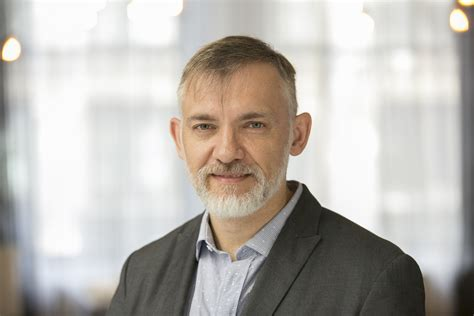
\includegraphics[scale=.13]{kapustin}
		\hspace*{1cm}
		
\includegraphics[scale=.21]{thorngren}
	\end{center}
	
	\pause
%	\vskip 20pt
	
	\begin{result}
		Effective construction of Adem coboundaries.
	\end{result}

	The above is joint with G. Brumfiel (Stanford) and J. Morgan (Columbia).
	
	\begin{center}
		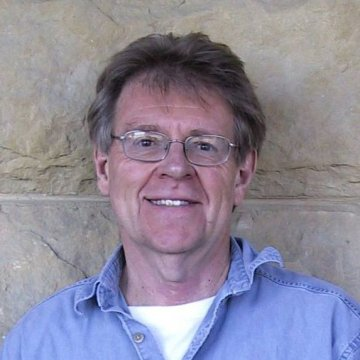
\includegraphics[scale=.21]{brumfiel}
		\hspace*{1cm}
		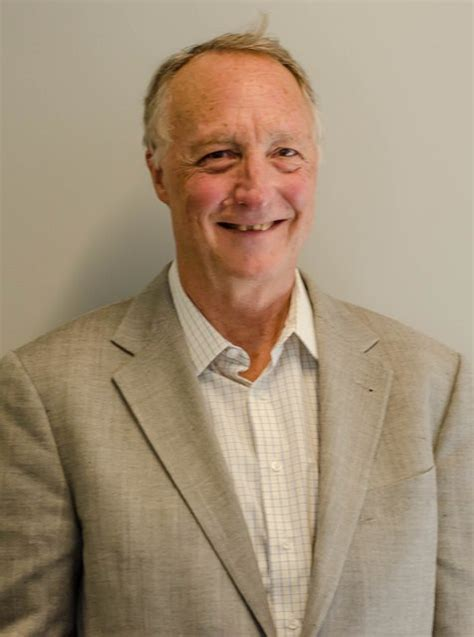
\includegraphics[scale=.09]{morgan}
	\end{center}
	
\end{frame}

\begin{frame}{Odd primes}
	
	So far we have focused on $\mathbb{F}_2$ coefficients.
	
	\vskip 5pt
	
	
	What about odd primes?
	
	\pause
	\vskip 5pt
	
	
	\begin{result}
		Effective construction of a generalization of the $\smallsmile_i$-products to coefficients in $\mathbb F_p$ for any prime $p$.
	\end{result}
	joint with R. Kaufmann (Purdue).
	
	\begin{center}
		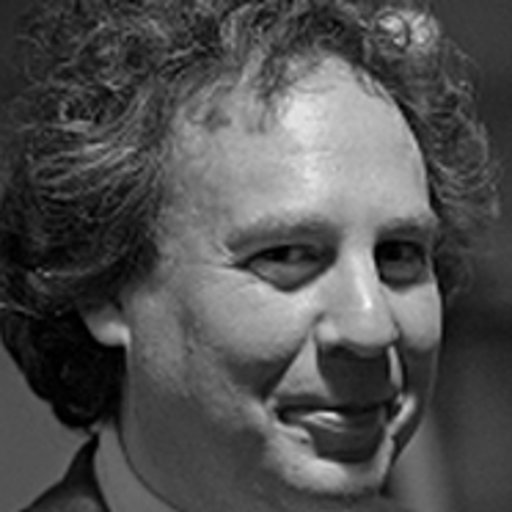
\includegraphics[scale=.1]{kaufmann}
	\end{center}
	
	\pause
	\vskip 9pt
	
	\textcolor{pblue}{What made these advances possible?}
	
\end{frame}

\section{The operadic point of view}

\begin{frame}{The renaissance of operads}
	
	Now a days we understand that the ``derived" version of a commutative algebra is an algebra over an $E_\infty$-operad (P. May).
	
	\vskip 10 pt
	\pause
	
	There are effective models due to McClure-Smith and Berger-Fresse.
	
	\begin{result}[M-M]
		A computer algebra system on Python for the study of these operads and their algebras. (Right place to implement some of the earlier results).
	\end{result}
	
	\vskip 10 pt
	\pause
	
	More theoretically,
	
	\begin{result}[M-M]
		Although no finitely presented $E_\infty$-operad can exist, I constructed a finitely presented prop $\mathcal M$ whose associated operad is $E_\infty$. Furthermore, \\
		this operad is cofibrant and compatible with previous algebraic models.		
	\end{result}
\end{frame}


%\section*{References}
%
%\begin{frame}[allowframebreaks]
%	\frametitle{References}
%	\nocite{whitney1935history}
%	\bibliographystyle{amsalpha}
%	\bibliography{biblio.bib}
%\end{frame}

\end{document}
